%(BEGIN_QUESTION)
% Copyright 2010, Tony R. Kuphaldt, released under the Creative Commons Attribution License (v 1.0)
% This means you may do almost anything with this work of mine, so long as you give me proper credit

Connect a potentiometer to the VFD in such a way that the pot's position controls the speed of the motor, rather than a knob or buttons on the VFD's front-panel.  You will need to research the VFD's User Manual both for determining where to connect the potentiometer as well as which parameter to change to make the VFD responsive to this external pot setting.

$$\includegraphics[width=15.5cm]{i04074x01.eps}$$

As always, your wire connections should be marshalled through terminal blocks (no taped or twisted wire joints!), with no bare copper showing at the connection points.

\vskip 20pt \vbox{\hrule \hbox{\strut \vrule{} {\bf Suggestions for Socratic discussion} \vrule} \hrule}

\begin{itemize}
\item{} Describe what the ``base'' parameters in a VFD refer to, and explain why these parameters are among the most important settings in the VFD.  Describe by way of illustration what may happen if these base parameters are set incorrectly.
\item{} Some large VFDs need to be ``gently'' powered up if they have been left un-powered for long periods of time, to avoid ``shocking'' the capacitors used to filter their DC busses.  Identify a means of doing so (i.e. limiting the inrush current that will occur when fully discharged capacitors are connected to a voltage source) that is easy and safe to implement.
\item{} Identify a practical application for a remote speed control such as this.
\end{itemize}

\underbar{file i04074}
%(END_QUESTION)




%(BEGIN_ANSWER)


%(END_ANSWER)





%(BEGIN_NOTES)


%INDEX% Final Control Elements, motor: variable frequency drive

%(END_NOTES)


